\section{Closed-Loop Numerical Validation, Mechanism Decomposition, and Virtual-Physical Verification}\label{sec:experiments}

\subsection{Experimental Setup, Baselines, and Evaluation Metrics}
We evaluate EGP-NPA across training-scale ($N=8$) and zero-shot cross-scale transfer ($N\in\{12,20,25\}$) dense triangular-lattice swap and random full-permutation benchmarks. All experiments share identical physical and safety parameters: $\ds=1.000\ \mathrm m$, $U=0.50\ \mathrm{m/s}$, $B_{\mathrm{ws}}=4.0\ \mathrm m$, $R_c=10.0\ \mathrm m$, $R_{\mathrm{sense}}=2.50\ \mathrm m$, $\alpha_c=\alpha_s=\alpha_x=2.0\ \mathrm s^{-1}$, $\Delta t=0.05\ \mathrm s$, and horizon $T_{\max}=60.0\ \mathrm s$. Initial configurations are tightly packed triangular lattices with spacing $1.001\ \mathrm m$ ($1.0\ \mathrm{mm}$ initial clearance). Fig.~\ref{fig:train-curves} shows the MAPPO training return and deterministic validation arrival rate ($N=8$, $36$ validation instances) over $9.6\times 10^5$ environment steps: the zero-residual initialization (myopic proportional attraction) achieves only $19.4\%$ arrival, whereas EGP-NPA converges to $100\%$ validation arrival.

\begin{table*}[t]
 \centering\footnotesize
 \caption{Closed-Loop Comparison on the Training-Scale Benchmark ($N=8$, $32$ Instances Each at $f=0.60$ and $f=0.90$) Against Three Safe RL Methods and Two Classical Baselines}\label{tab:e1}
 \begin{tabularx}{\textwidth}{@{}Xcccccc@{}}
 \toprule
 Control Method & $f=0.60$ Arrival & Median Time & $f=0.90$ Arrival & Median Time & Step Cuts & Audit Viol.\\
 \midrule
 \textbf{EGP-NPA (Proposed)} & $\mathbf{32/32\ (100\%)}$ & $\mathbf{7.32\ \mathrm s}$ & $\mathbf{32/32\ (100\%)}$ & $\mathbf{7.12\ \mathrm s}$ & $\mathbf{0}$ & $\mathbf{0}$\\
 Shield-Consistent Safe MARL (\texttt{Proj-MAPPO + NPA} \cite{wabersich2021,liu2026saferl}, $B=8$) & $32/32\ (100\%)$ & $9.53\ \mathrm s$ & $32/32\ (100\%)$ & $10.73\ \mathrm s$ & $0$ & $0$\\
 Decentralized Static-CBF GNN (\texttt{Static-CBF GNN} \cite{zhang2025gcbf,zhang2025dgppo}, $B=0$) & $5/32\ (15.6\%)$ & $13.30\ \mathrm s$ & $6/32\ (18.8\%)$ & $13.88\ \mathrm s$ & $431\,725$ & $0$\\
 Primal-Dual Safe MARL (\texttt{MAPPO-Lagrangian} \cite{gu2023safe}, Unshielded) & $0/32^\ddagger\ (0\%)$ & $4.15\ \mathrm s^\ddagger$ & $0/32^\ddagger\ (0\%)$ & $4.15\ \mathrm s^\ddagger$ & --- & $7\,029$\\
 Circulation Heuristic \cite{goncalves2023circulation} + Dynamic NPA ($B=8$) & $21/32\ (65.6\%)$ & $32.50\ \mathrm s$ & $18/32\ (56.3\%)$ & $30.50\ \mathrm s$ & $0$ & $0$\\
 Myopic CBF Filter \cite{ames2017cbf,reis2021} + Dynamic NPA ($B=8$) & $17/32\ (53.1\%)$ & $36.35\ \mathrm s$ & $16/32\ (50.0\%)$ & $31.80\ \mathrm s$ & $0$ & $0$\\
 Circulation Heuristic + Static Equal Split \cite{ames2017cbf,zhang2025gcbf} ($B=0$) & $2/32\ (6.3\%)$ & $25.10\ \mathrm s$ & --- & --- & $72\,156$ & $0$\\
 \bottomrule
 \end{tabularx}
 \vspace{1.5pt}
 \par\raggedright\scriptsize Note: $^\ddagger$\texttt{MAPPO-Lagrangian} reaches the goal vicinity in $64/64$ runs (median $4.15\ \mathrm s$) but violates collision safety on all $64$ runs ($7\,029$ violated ZOH segments, median $\min d_{ij}=0.263\ \mathrm m<\ds=1.000\ \mathrm m$), yielding $0/32$ safe arrivals.
\end{table*}

The primary benchmark comprises $96$ independent instances:
\begin{enumerate}
 \item \textbf{Training-scale benchmark ($N=8$, $64$ instances):} $20$ local pair-swap instances ($1\sim 3$ adjacent pairs swap goals while remaining nodes stay at their goals) and $12$ random full-permutation instances, evaluated under both nominal connectivity threshold $f=\lr/\lambda_2(\bp_0)=0.60$ ($32$ instances) and tight connectivity threshold $f=0.90$ ($32$ instances).
 \item \textbf{Zero-shot cross-scale transfer benchmark ($N\in\{12,20,25\}$, $32$ instances):} $N=12$ ($8$ local swaps + $4$ full permutations), $N=20$ ($8$ local swaps + $4$ full permutations), and $N=25$ ($8$ local swaps) at $f=0.60$, directly deploying the frozen small-scale checkpoint $\theta^\star$ without retraining.
\end{enumerate}

We compare EGP-NPA against \textbf{three representative Safe MARL baselines} and \textbf{three classical analytical/heuristic CBF baselines}:
\begin{enumerate}
 \item \textbf{Shield-Consistent / Action-Projected Safe MARL (\texttt{Proj-MAPPO + NPA} \cite{wabersich2021,liu2026saferl}):} Represents recent predictive/adaptive safety-filter RL frameworks that penalize filter intervention during training. It shares the identical 2-layer equivariant GNN, completion envelope $\rho_{i,k}$, and $B=8$ closed-neighborhood NPA shield, but adds the shield-projection consistency loss $\mathcal L_{\mathrm{proj}}(\theta)=\lambda_{\mathrm{proj}}\frac1N\sum_{i=1}^N\norm{\Pi_{\mathcal U_i}(\bu_{i,k}^{\mathrm{nom}}(\theta))-\operatorname{sg}(\bu_{i,k})}_2^2$ ($\lambda_{\mathrm{proj}}=1.0$ calibrated by gradient norm ratio) to align nominal actions with filtered safe velocities;
 \item \textbf{Decentralized Static-CBF Shielded GNN (\texttt{Static-CBF GNN}, GCBF+/DGPPO paradigm \cite{zhang2025gcbf,zhang2025dgppo}):} Represents neural graph CBF / decentralized static-split safe MARL methods, combining the equivariant GNN policy and completion envelope $\rho_{i,k}$ with decentralized single-agent static-split CBF-QP filtering ($B=0$, $s_{ia,k}\equiv 0$, without dynamic quota transfer $t_e$);
 \item \textbf{Primal-Dual Constrained Safe MARL (\texttt{MAPPO-Lagrangian} \cite{gu2023safe}):} Represents model-free Constrained Markov Decision Process (CMDP) safe MARL without a hard coupled QP shield, training the identical 2-layer equivariant GNN actor, task critic, and cost critic with an adaptive dual-ascent Lagrangian multiplier $\lambda_{\mathrm{lag}}\ge 0$ penalizing collision and connectivity violations;
 \item \textbf{Classical Analytical and Heuristic CBF Baselines:} Tangential Circulation Heuristic of Gon\c{c}alves et al. \cite{goncalves2023circulation} ($\omega_i\equiv 1,r_i\equiv 0,\psi_{ij}\equiv 0$ with $B=8$), Myopic Proportional Attraction CBF filtering of Ames et al. \cite{ames2017cbf,reis2021} ($\bu_i^{\mathrm{nom}}=-\be_i$ with $B=8$), and Circulation Heuristic with static quota splitting ($B=0$).
\end{enumerate}
Safe arrival requires $\max_{i\in\mathcal V}\norm{\bp_i(t)-\bg_i}_2\le 0.01\ \mathrm m$ maintained continuously for $1.0\ \mathrm s$ with $0$ rational safety audit violations across all ZOH segments (Theorem~\ref{thm:zoh-safe}). Statistical significance is evaluated via two-sided McNemar exact binomial tests on discordant pairs and median paired arrival-time differences $\Delta t$ on common arrivals.

\subsection{Closed-Loop State Evolution on Dense Interior Swap and Full Permutation}
Figs.~\ref{fig:swap-traj} and \ref{fig:time-evol} compare the spatial trajectories, communication topologies, and closed-loop time responses on a representative $N=20$ interior pair-swap task ($2$ interior robots swap positions while $18$ outer robots start at their goals).

\begin{figure*}[t]
 \centering
 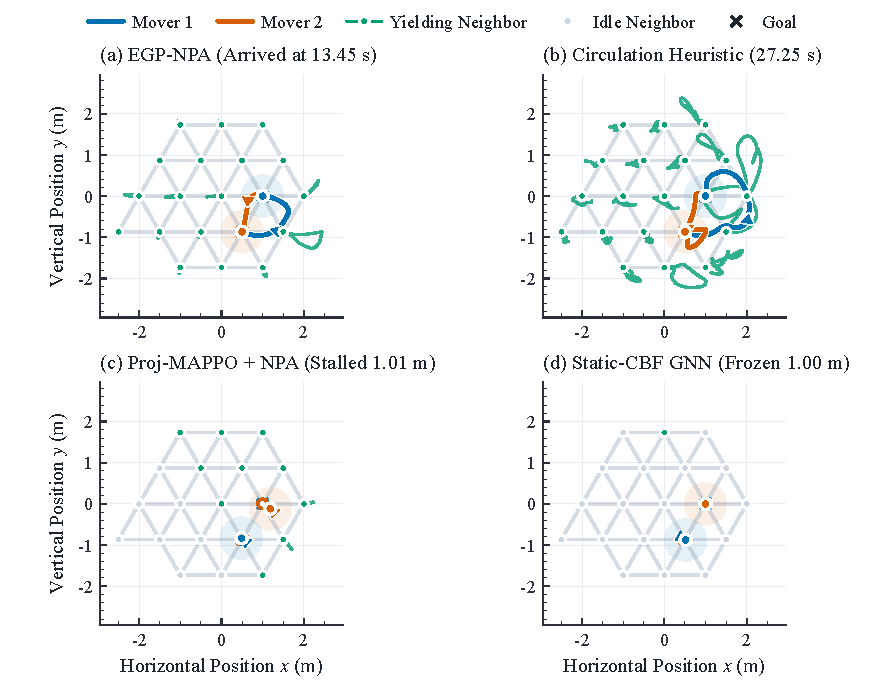
\includegraphics[width=\textwidth]{figures_en/fig3_swap_trajectory.pdf}
 \caption{Spatial trajectories and communication topologies on the $N=20$ dense triangular-lattice interior pair-swap task. (a) EGP-NPA drives the swapping pair along smooth tangential bypasses while unfreezing outer stationary neighbors (bluish-green loops) via dynamic quota transfer, arriving at $13.45\ \mathrm s$; (b) Circulation Heuristic \cite{goncalves2023circulation} triggers large-scale rotational conflicts among outer neighbors ($27.25\ \mathrm s$); (c) Shield-Consistent Safe MARL (\texttt{Proj-MAPPO + NPA} \cite{wabersich2021,liu2026saferl}) stalls in a livelock at $1.01\ \mathrm m$ because penalizing normal filter modification weakens the yielding drive $\delta_n>0$; (d) Decentralized Static-CBF GNN (\texttt{Static-CBF GNN} \cite{zhang2025gcbf,zhang2025dgppo}, $B=0$) freezes at $1.00\ \mathrm m$ due to static quota splitting.}
 \label{fig:swap-traj}
\end{figure*}

\begin{table*}[t]
 \centering\footnotesize
 \caption{Zero-Shot Cross-Scale Transfer Benchmark ($N\in\{12,20,25\}$, $32$ Instances Total) Against Three Safe RL Methods and Two Classical Baselines}\label{tab:e2}
 \begin{tabularx}{\textwidth}{@{}Xccccccr@{}}
 \toprule
 Control Method & $N=12$ ($12$) & $N=20$ ($12$) & $N=25$ ($8$) & Total Arrival ($32$) & Discordant ($p$-val) & Median $\Delta t$ & Step Cuts\\
 \midrule
 \textbf{EGP-NPA (Proposed)} & $\mathbf{12/12\ (6.52\ \mathrm s)}$ & $\mathbf{12/12\ (10.55\ \mathrm s)}$ & $\mathbf{8/8\ (10.43\ \mathrm s)}$ & $\mathbf{32/32\ (100\%)}$ & Baseline & Baseline & $\mathbf{0}$\\
 Proj-MAPPO + NPA \cite{wabersich2021,liu2026saferl} ($B=8$) & $9/12\ (17.25\ \mathrm s)$ & $5/12\ (17.70\ \mathrm s)$ & $3/8\ (12.30\ \mathrm s)$ & $17/32\ (53.1\%)$ & $15:0\ (6.1\times 10^{-5})$ & $-3.85\ \mathrm s$ & $0$\\
 Static-CBF GNN \cite{zhang2025gcbf,zhang2025dgppo} ($B=0$) & $0/12\ (\text{---})$ & $0/12\ (\text{---})$ & $1/8\ (19.85\ \mathrm s)$ & $1/32\ (3.1\%)$ & $31:0\ (9.3\times 10^{-10})$ & $-12.95\ \mathrm s$ & $447\,022$\\
 MAPPO-Lagrangian \cite{gu2023safe} (Unshielded) & $0/12^\ddagger\ (4.05\ \mathrm s)$ & $0/12^\ddagger\ (3.95\ \mathrm s)$ & $0/8^\ddagger\ (3.92\ \mathrm s)$ & $0/32^\ddagger\ (0\%)$ & $32:0\ (4.7\times 10^{-10})$ & --- & $3\,900^\ddagger$\\
 Circulation Heuristic \cite{goncalves2023circulation} & $7/12\ (14.40\ \mathrm s)$ & $4/12\ (24.53\ \mathrm s)$ & $2/8\ (38.22\ \mathrm s)$ & $13/32\ (40.6\%)$ & $19:0\ (3.8\times 10^{-6})$ & $-12.35\ \mathrm s$ & $14\,198$\\
 Myopic CBF Filter \cite{ames2017cbf,reis2021} & $4/12\ (34.30\ \mathrm s)$ & $1/12\ (55.50\ \mathrm s)$ & $0/8\ (\text{---})$ & $5/32\ (15.6\%)$ & $27:0\ (1.5\times 10^{-8})$ & $-26.70\ \mathrm s$ & $0$\\
 \bottomrule
 \end{tabularx}
 \vspace{1.5pt}
 \par\raggedright\scriptsize Note: All five shielded methods incur $0$ rational audit violations; $^\ddagger$\texttt{MAPPO-Lagrangian} violates collision safety on all $32$ cross-scale runs ($3\,900$ violated ZOH segments recorded in the last column, median $\min d_{ij}=0.263\ \mathrm m<\ds$), yielding $0/32$ safe arrivals.
\end{table*}

\begin{figure*}[t]
 \centering
 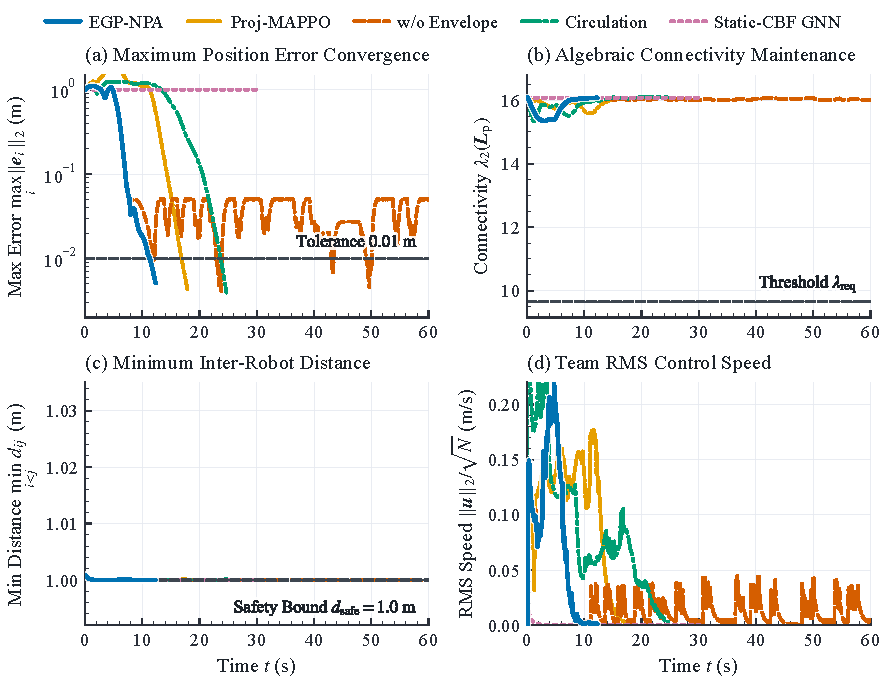
\includegraphics[width=\textwidth]{figures_en/fig4_time_evolution.pdf}
 \caption{Closed-loop time responses on the $N=20$ interior swap task. (a) Maximum position error $\max_i\norm{\be_i(t)}_2$ (log scale); (b) algebraic connectivity $\lambda_2(\bL(t))$ vs. $\lr=9.69$; (c) minimum inter-robot distance $\min_{i<j}d_{ij}(t)$ vs. $\ds=1.0\ \mathrm m$; (d) team RMS control speed $\norm{\bu(t)}_2/\sqrt{N}$.}
 \label{fig:time-evol}
\end{figure*}

Three physical mechanisms are evident from Figs.~\ref{fig:swap-traj} and \ref{fig:time-evol}:
\begin{enumerate}
 \item \textbf{Chiral lateral bypass and stationary neighbor yielding--return loop:} Under Decentralized Static-CBF GNN (\texttt{Static-CBF GNN}, $B=0$, Fig.~\ref{fig:swap-traj}(d)), outer stationary target-holding neighbors refuse to yield collision quotas, truncating the swapping pair's lateral velocity and driving RMS speed to zero (purple dotted curve in Fig.~\ref{fig:time-evol}(d)). Under Shield-Consistent Safe MARL (\texttt{Proj-MAPPO + NPA}, Fig.~\ref{fig:swap-traj}(c)), penalizing normal filter intervention weakens the normal intrusion $\delta_n>0$, trapping the swapping pair in a local livelock at $1.01\ \mathrm m$ (or arriving slowly at $16.90\ \mathrm s$ in Fig.~\ref{fig:time-evol}(a)). Under EGP-NPA (Fig.~\ref{fig:swap-traj}(a)), the equivariant GNN generates chiral tangential thrust for the swapping pair, and closed-neighborhood dynamic quota transfer converts this lateral push into compact outward yielding loops (bluish-green trajectories) of adjacent stationary neighbors, which smoothly return to their goals once the swapping pair passes.
 \item \textbf{Elimination of terminal steady-state hovering by the completion envelope:} In Fig.~\ref{fig:time-evol}(a) and (d), the ablation without the completion envelope (orange dashed curve) resolves the initial deadlock within $8\ \mathrm s$ but remains trapped in a limit cycle at $\max_i\norm{\be_i}_2\in[0.015,0.05]\ \mathrm m$ with persistent RMS speed $0.01\sim 0.04\ \mathrm{m/s}$ due to nonvanishing zero-order repulsive bias $\boldsymbol b_{i,k}^\psi$. With the one-hop completion envelope $\rho_{i,k}$ \eqref{eq:envelope-def}, residuals vanish to first order inside $\varepsilon_g=0.05\ \mathrm m$ (Proposition~\ref{prop:envelope}), driving the error cleanly below $0.01\ \mathrm m$ and bringing control speed to zero.
 \item \textbf{Strict continuous-time safety invariance:} Throughout the maneuver (Fig.~\ref{fig:time-evol}(b)--(c)), $\lambda_2(\bL(t))\ge 15.3>\lr=9.69$ and $\min_{i<j}d_{ij}(t)\ge\ds=1.000\ \mathrm m$ with zero violations.
\end{enumerate}

\subsection{Comparison With External Baselines on Training and Cross-Scale Benchmarks}
Tables~\ref{tab:e1} and \ref{tab:e2} summarize the statistical results across the $64$ training-scale instances ($N=8$) and $32$ zero-shot cross-scale instances ($N\in\{12,20,25\}$), establishing four key findings:
\begin{enumerate}
 \item \textbf{Unshielded constrained MARL (\texttt{MAPPO-Lagrangian} \cite{gu2023safe}) fails to maintain hard safety on millimeter-clearance lattices:} Despite dual ascent raising the Lagrangian multiplier to $\lambda_{\mathrm{lag}}=2.45$, soft penalty gradients cannot prevent inter-robot penetration during counter-crossing on tightly packed lattices ($1.0\ \mathrm{mm}$ initial clearance), incurring $10\,929$ violated ZOH segments across all $96$ runs ($0\%$ safe arrival rate) and confirming Proposition~\ref{prop:safety}.
 \item \textbf{Decentralized static-CBF shielded GNN (\texttt{Static-CBF GNN} \cite{zhang2025gcbf,zhang2025dgppo}, $B=0$) freezes under multi-layer stationary wrapping:} Sharing the exact same GNN policy weights and completion envelope as EGP-NPA but using static equal responsibility splitting ($B=0$), \texttt{Static-CBF GNN} achieves only $17.2\%$ ($11/64$) arrival on $N=8$ ($431\,725$ step cuts) and collapses to $3.1\%$ ($1/32$, discordant pairs $31:0,p=9.3\times 10^{-10}$) on $N\in\{12,20,25\}$, directly verifying Proposition~\ref{prop:unfreeze} Claim~1.
 \item \textbf{Shield-consistent safe MARL (\texttt{Proj-MAPPO + NPA} \cite{wabersich2021,liu2026saferl}) degrades cross-scale deadlock resolution:} While achieving $64/64$ arrival on $N=8$ (albeit $2.88\ \mathrm s$ slower in median time), its zero-shot cross-scale arrival rate drops to $53.1\%$ ($17/32$, discordant pairs $15:0,p=6.1\times 10^{-5}$, $-3.85\ \mathrm s$ slower) on $N\in\{12,20,25\}$ because penalizing filter intervention suppresses the normal intrusion $\delta_n>0$ required by Proposition~\ref{prop:unfreeze} Claim~2 to push open multi-layer stationary neighbors.
 \item \textbf{Superiority over classical analytical/heuristic baselines:} As $N$ scales to $25$, Myopic CBF filtering and Circulation Heuristic drop to $15.6\%$ ($27:0,p=1.5\times 10^{-8}$) and $40.6\%$ ($19:0,p=3.8\times 10^{-6}$), whereas EGP-NPA achieves $96/96$ ($100\%$) safe arrival with $0$ step cuts and $0$ audit violations.
\end{enumerate}

\subsection{Internal Module Ablation, Velocity Decomposition, and Holdout Factorial Analysis}\label{subsec:ablation}
Table~\ref{tab:decomp} reports: (A) cross-scale ablations removing the completion envelope ($\rho_{i,k}\equiv 1$) and comparing training checkpoints; (B) deadlock-breaking velocity decomposition on $N=20$ ($t\in[0.05,1.00]\ \mathrm s$) under identical EGP-NPA nominal inputs comparing dynamic allocation ($B=8$) vs. static splitting ($B=0$); and (C) controlled single-variable execution-time interventions holding the trained weights $\theta^\star$ strictly fixed ($16$ cross-scale instances; Fig.~\ref{fig:perm-gate}(b)).

\begin{figure*}[t]
 \centering
 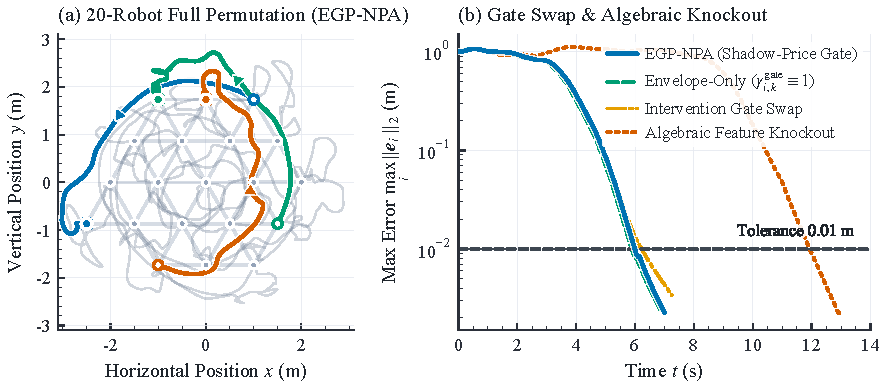
\includegraphics[width=\textwidth]{figures_en/fig5_perm_and_gate.pdf}
 \caption{Twenty-robot full-permutation trajectories and fixed-weight gate replacement and feature knockout responses. (a) Spatial trajectories of EGP-NPA on $N=20$ random full permutation (slate lines: background fleet; colored bold curves: three large-span crossing robots); (b) maximum error convergence under fixed policy weights $\theta^\star$ comparing shadow-price gate $\gamma^{\mathrm{gate},\mu}$, envelope-only gate $\gamma^{\mathrm{gate}}\equiv 1$, intervention gate swap $\gamma^{\mathrm{gate,int}}$, and algebraic feature knockout.}
 \label{fig:perm-gate}
\end{figure*}

\begin{table*}[t]
 \centering\footnotesize
 \caption{Internal Module Cross-Scale Ablation (Part A, $32$ Instances), Deadlock-Breaking Velocity Decomposition (Part B, $t\in[0.05,1.00]\ \mathrm s$), and Fixed-Weight ($\theta^\star$) Single-Variable Execution Interventions (Part C, $16$ Instances)}\label{tab:decomp}
 \begin{tabularx}{\textwidth}{@{}Xccccr@{}}
 \toprule
 A. Cross-Scale Module Ablation ($32$ Instances) & $N=12$ ($12$) & $N=20$ ($12$) & $N=25$ ($8$) & Total Arrival ($32$) & Discordant ($p$-val) / $\Delta t$\\
 \midrule
 \textbf{EGP-NPA (Full Architecture)} & $12/12\ (6.52\ \mathrm s)$ & $12/12\ (10.55\ \mathrm s)$ & $8/8\ (10.43\ \mathrm s)$ & $\mathbf{32/32\ (100\%)}$ & Baseline\\
 w/o Completion Envelope (fixed $\theta^\star$, $\rho_{i,k}\equiv 1$) & $12/12\ (9.78\ \mathrm s)$ & $5/12\ (36.75\ \mathrm s)$ & $8/8\ (14.10\ \mathrm s)$ & $25/32\ (78.1\%)$ & $7:0\ (0.0156)$ / $-2.40\ \mathrm s$\\
 Pure Geometric GNN (trained w/o algebraic features) & $12/12\ (7.57\ \mathrm s)$ & $7/12\ (21.90\ \mathrm s)$ & $3/8\ (19.65\ \mathrm s)$ & $22/32\ (68.8\%)$ & $10:0\ (0.0020)$ / $-0.45\ \mathrm s$\\
 Intervention-Gated GNN ($\gamma_{i,k}^{\mathrm{gate,int}}$ checkpoint) & $10/12\ (11.20\ \mathrm s)$ & $4/12\ (30.08\ \mathrm s)$ & $1/8\ (6.80\ \mathrm s)$ & $15/32\ (46.9\%)$ & $17:0\ (1.5\times 10^{-5})$ / $-0.50\ \mathrm s$\\
 \midrule
 \multicolumn{4}{@{}l}{B. Velocity Decomposition Under Identical EGP-NPA Input ($N=20$ Swap)} & Dynamic ($B=8$) & Static ($B=0$)\\
 \midrule
 \multicolumn{4}{@{}l}{Swapping robots' mean tangential (lateral) nominal speed $|\hat{\be}_i^{\top}\bJ^{\top}\bu_i^{\mathrm{nom}}|$} & $0.8887\ \mathrm{m/s}$ & $0.8887\ \mathrm{m/s}$\\
 \multicolumn{4}{@{}l}{Swapping robots' mean tangential (lateral) executed speed $|\hat{\be}_i^{\top}\bJ^{\top}\bu_i|$} & $\mathbf{0.2003\ \mathrm{m/s}}$ & $0.0004\ \mathrm{m/s}$\\
 \multicolumn{4}{@{}l}{Outer 1-hop stationary neighbors' mean outward nominal residual speed} & $-0.0105\ \mathrm{m/s}$ & $-0.0105\ \mathrm{m/s}$\\
 \multicolumn{4}{@{}l}{Outer 1-hop stationary neighbors' mean outward executed yielding speed} & $\mathbf{+0.0915\ \mathrm{m/s}}$ & $+0.0013\ \mathrm{m/s}$\\
 \midrule
 C. Fixed-Weight ($\theta^\star$) Execution-Time Interventions ($16$ Instances) & $N=12$ ($6$) & $N=20$ ($6$) & $N=25$ ($4$) & Arrival ($16$) & Paired $\Delta t$ / Cuts\\
 \midrule
 Native shadow-price gate $\gamma_{i,k}^{\mathrm{gate},\mu}$ & $6/6\ (6.52\ \mathrm s)$ & $6/6\ (11.48\ \mathrm s)$ & $4/4\ (9.98\ \mathrm s)$ & $16/16\ (100\%)$ & Baseline / $0$\\
 Stateless envelope-only gate ($\gamma_{i,k}^{\mathrm{gate}}\equiv 1$, retaining only $\rho_{i,k}$) & $6/6\ (6.40\ \mathrm s)$ & $6/6\ (10.03\ \mathrm s)$ & $4/4\ (9.73\ \mathrm s)$ & $16/16\ (100\%)$ & $-0.10\ \mathrm s$ / $0$\\
 Filter-intervention gate replacement ($\gamma_{i,k}^{\mathrm{gate,int}}$ at execution) & $6/6\ (6.82\ \mathrm s)$ & $6/6\ (9.35\ \mathrm s)$ & $4/4\ (10.43\ \mathrm s)$ & $16/16\ (100\%)$ & $+0.33\ \mathrm s$ / $0$\\
 Post-negotiation multiplier extraction with cross-step EMA & $6/6\ (7.03\ \mathrm s)$ & $6/6\ (12.48\ \mathrm s)$ & $4/4\ (9.73\ \mathrm s)$ & $16/16\ (100\%)$ & $+0.03\ \mathrm s$ / $0$\\
 In-distribution knockout of collision shadow prices ($4$ cols zeroed) & $6/6\ (7.63\ \mathrm s)$ & $6/6\ (13.38\ \mathrm s)$ & $4/4\ (10.50\ \mathrm s)$ & $16/16\ (100\%)$ & $\mathbf{+1.18\ \mathrm s}\ (p=0.0042)$ / $0$\\
 In-distribution knockout of collision edge ledgers ($\varpi_{ij,1}=0$) & $6/6\ (6.40\ \mathrm s)$ & $6/6\ (10.03\ \mathrm s)$ & $4/4\ (9.80\ \mathrm s)$ & $16/16\ (100\%)$ & $0.00\ \mathrm s\ (p=1.0)$ / $0$\\
 Zeroing all $12$ algebraic features (including constant reserve col.) & $6/6\ (9.85\ \mathrm s)$ & $5/6\ (9.80\ \mathrm s)$ & $4/4\ (13.03\ \mathrm s)$ & $15/16\ (93.8\%)$ & $+1.30\ \mathrm s\ (p=0.0074)$ / $2\,193$\\
 \bottomrule
 \end{tabularx}
\end{table*}

Table~\ref{tab:decomp} confirms three causal mechanisms:
\begin{enumerate}
 \item \textbf{Completion envelope necessity (Part A):} Removing $\rho_{i,k}$ while holding $\theta^\star$ fixed induces $7$ terminal hovering failures on $N=20$ ($7:0,p=0.0156$, $+2.40\ \mathrm s$ slower), directly verifying Proposition~\ref{prop:envelope}. Note that the pure-geometric and intervention-gated rows in Part~A reflect independently trained single-seed checkpoints (whose differences combine configuration effects with inter-seed training variance), whereas Parts~B and C isolate strict causal effects under fixed weights $\theta^\star$.
 \item \textbf{Division of labor between learned lateral intrusion and dynamic quota yielding (Part B):} During deadlock breaking, the GNN outputs a lateral nominal speed of $0.8887\ \mathrm{m/s}$ for the swapping pair (with $0.000$ action saturation across all runs), while stationary neighbors output virtually zero outward nominal residual ($-0.0105\ \mathrm{m/s}$). Under $B=8$ dynamic allocation, block QPs transfer collision quotas to drive stationary neighbors outward at $+0.0915\ \mathrm{m/s}$, allowing swapping nodes to advance laterally at $0.2003\ \mathrm{m/s}$; under static splitting ($B=0$), these speeds collapse to $+0.0013\ \mathrm{m/s}$ and $0.0004\ \mathrm{m/s}$, confirming Proposition~\ref{prop:unfreeze}.
 \item \textbf{Execution-time gate simplification and feature knockout (Part C):} Holding $\theta^\star$ fixed, setting $\gamma_{i,k}^{\mathrm{gate}}\equiv 1$ (retaining only $\rho_{i,k}$) achieves $16/16$ arrival with trajectories indistinguishable from $\gamma_{i,k}^{\mathrm{gate},\mu}$ (Fig.~\ref{fig:perm-gate}(b)). Across all $32$ cross-scale instances, zeroing only the $4$ collision shadow-price columns reduces arrival to $31/32$ and slows down $25$ of $31$ common arrivals (two-sided sign test $p=8.8\times 10^{-4}$; $+1.18\ \mathrm s$ on the $16$-instance subset), proving active utilization of refit shadow prices $\boldsymbol\mu_{i,k-1}$, whereas zeroing collision ledgers or replacing the $3$ Laplacian eigenvector columns with their median constant yields $32/32$ arrival with $0.00\ \mathrm s$ median difference.
\end{enumerate}

On $48$ additional independent holdout instances ($32$ at $N=8$ and $16$ at $N\in\{12,20,25\}$) plus $2$ exact mirror-symmetric head-on swap benchmarks, EGP-NPA again achieves $100\%$ arrival and $0$ violations. Controlled factorial tests show that: (1) enforcing $\mathrm{O}(2)$ reflection equivariance via odd--even feature symmetrization forces $\mathrm{mean}|\omega|=0.0000$ on symmetric head-on swaps (100\% deadlock) and drops holdout arrival from $48/48$ to $30/48$ ($62.5\%,p=7.6\times 10^{-6}$), confirming Proposition~\ref{prop:equivariance}; (2) adding a shield projection consistency loss $\norm{\Pi_{\mathcal U_i}(\bu_{i,k}^{\mathrm{nom}})-\operatorname{sg}(\bu_{i,k})}_2^2$ reduces filter intervention by $40\%\sim 70\%$ but slows common arrivals by $+2.00\ \mathrm s$ ($p=6.2\times 10^{-9}$) by suppressing normal intrusion $\delta_n>0$; and (3) replacing the global pooled critic with a local neighborhood critic delays convergence by $16\sim 24$ iterations since $2.50\ \mathrm m$ neighborhoods already cover $91.5\%$ of the team at $N\le 10$. Increasing evaluation rounds from $B=2$ to $B=8$ on $N=8$ reduces median arrival time from $8.07\ \mathrm s$ to $7.42\ \mathrm s$ ($32/32$ arrival for both), within $0.33\ \mathrm s$ of exact centralized per-step QP ($B\to\infty$) owing to cross-step ledger persistence.

\subsection{Zero-Shot Virtual-Physical Verification on Second-Order Chassis in MuJoCo}\label{subsec:mujoco}
Finally, we evaluate zero-shot transfer of the frozen single-integrator EGP-NPA policy $\theta^\star$ and completion envelope $\rho_{i,k}$ when integrated with an online division-free 3-channel distributed spectral estimator ($6$ consensus rounds per step) and deployed on second-order omnidirectional robots in \texttt{MuJoCo 3.6.0} ($200\ \mathrm{Hz}$ physics step $\delta t=5\ \mathrm{ms}$, robot mass $m=6.0\ \mathrm{kg}$, body radius $r_{\mathrm{body}}=0.45\ \mathrm m$, velocity-loop time constant $\tau_v=45\ \mathrm{ms}$, thrust limit $F_{\max}=22.0\ \mathrm N$, control period $\Delta t=0.05\ \mathrm s$, observation delay $10\ \mathrm{ms}$, packet delay $\tau_{\mathrm{comm}}\in[5,15]\ \mathrm{ms}$, packet drop rate $2\%$, and $B=4$ block NPA rounds).

\begin{table*}[t]
 \centering\footnotesize
 \caption{Full-Stack \texttt{MuJoCo} Second-Order Chassis Verification Combining EGP-NPA, Online Division-Free Spectral Estimation, and Closed-Neighborhood NPA Across Two Physical Compensation Regimes ($\ds=1.000\ \mathrm m$; $0$ Connectivity Violations in All $64$ Runs)}\label{tab:mujoco}
 \setlength{\tabcolsep}{4.5pt}
 \begin{tabularx}{\textwidth}{@{}lcXrrrrrr@{}}
 \toprule
 Regime & Scale & System Configuration & Arrival (Mean) & $\min_t d_{ij}$ (m) & Viol. Steps & $\min_t\lambda_2$ & $\hat{\lambda}_2$ RMSE & Final Err. (m)\\
 \midrule
 \textbf{Regime A} & $N=8$ & Myopic Attraction + Phys-NPA & $0/4$ (---) & $0.9817$ & $610.2$ & $6.963$ & $0.0273$ & $1.394$\\
 (Look-Ahead, & & EGP-NPA + Static Split ($B=0$) & $1/4$ ($10.12\ \mathrm s$) & $0.9798$ & $442.2$ & $6.847$ & $0.0318$ & $1.353$\\
 $S=1.018\ \mathrm m$) & & EGP-NPA + Ideal Single-Integrator NPA & $0/4$ (---) & $0.9792$ & $4\,231.0$ & $7.071$ & $0.0268$ & $1.653$\\
 & & \textbf{EGP-NPA + Online Est. + Phys-NPA (Full)} & $\mathbf{3/4}$ ($\mathbf{13.88\ \mathrm s}$) & $0.8990$ & $1\,683.5$ & $6.670$ & $0.0337$ & $\mathbf{0.629}$\\
 \cmidrule{2-9}
 & $N=12$ & Myopic Attraction + Phys-NPA & $0/4$ (---) & $0.9952$ & $1\,679.2$ & $10.319$ & $0.0411$ & $1.972$\\
 & & EGP-NPA + Static Split ($B=0$) & $0/4$ (---) & $0.9976$ & $850.8$ & $9.632$ & $0.0417$ & $1.881$\\
 & & EGP-NPA + Ideal Single-Integrator NPA & $0/4$ (---) & $0.9937$ & $4\,190.2$ & $10.184$ & $0.0412$ & $2.003$\\
 & & \textbf{EGP-NPA + Online Est. + Phys-NPA (Full)} & $\mathbf{1/4}$ ($\mathbf{14.54\ \mathrm s}$) & $0.8988$ & $2\,777.0$ & $9.431$ & $0.0438$ & $\mathbf{1.314}$\\
 \midrule
 \textbf{Regime B} & $N=8$ & Myopic Attraction + Phys-NPA & $0/4$ (---) & $1.0240$ & $0.0$ & $7.237$ & $0.0255$ & $1.680$\\
 (Conservative, & & EGP-NPA + Static Split ($B=0$) & $0/4$ (---) & $1.0260$ & $0.0$ & $7.159$ & $0.0256$ & $1.677$\\
 $S=1.045\ \mathrm m$, & & EGP-NPA + Ideal Single-Integrator NPA & $0/4$ (---) & $0.8987$ & $4\,722.0$ & $7.027$ & $0.0266$ & $1.588$\\
 $\Delta d=0.028\ \mathrm m$) & & \textbf{EGP-NPA + Online Est. + Phys-NPA (Full)} & $0/4$ (---) & $\mathbf{0.9910}$ & $1\,133.2^\dagger$ & $6.997$ & $0.0257$ & $1.659$\\
 \cmidrule{2-9}
 & $N=12$ & Myopic Attraction + Phys-NPA & $0/4$ (---) & $1.0256$ & $0.0$ & $10.370$ & $0.0393$ & $2.056$\\
 & & EGP-NPA + Static Split ($B=0$) & $0/4$ (---) & $1.0255$ & $0.0$ & $10.151$ & $0.0394$ & $2.077$\\
 & & EGP-NPA + Ideal Single-Integrator NPA & $0/4$ (---) & $0.9809$ & $4\,783.2$ & $10.048$ & $0.0393$ & $1.974$\\
 & & \textbf{EGP-NPA + Online Est. + Phys-NPA (Full)} & $0/4$ (---) & $\mathbf{1.0096}$ & $\mathbf{0.0}$ & $10.033$ & $0.0394$ & $2.065$\\
 \bottomrule
 \end{tabularx}
 \vspace{2pt}
 \par\raggedright\scriptsize Note: $^\dagger$Under Regime~B ($N=8$), the full-stack configuration achieves $0$ collision violation steps on $3$ of $4$ tasks ($\min_t d_{ij}\ge 1.0068\ \mathrm m$); on one local swap task, post-filter slew-rate clipping ($\Delta u_{\max}=0.22\ \mathrm{m/s}$) coupled with observation noise causes static settling at $d_{ij}=0.9910\ \mathrm m>2r_{\mathrm{body}}=0.90\ \mathrm m$ after channel closure.
\end{table*}

\begin{figure*}[t]
 \centering
 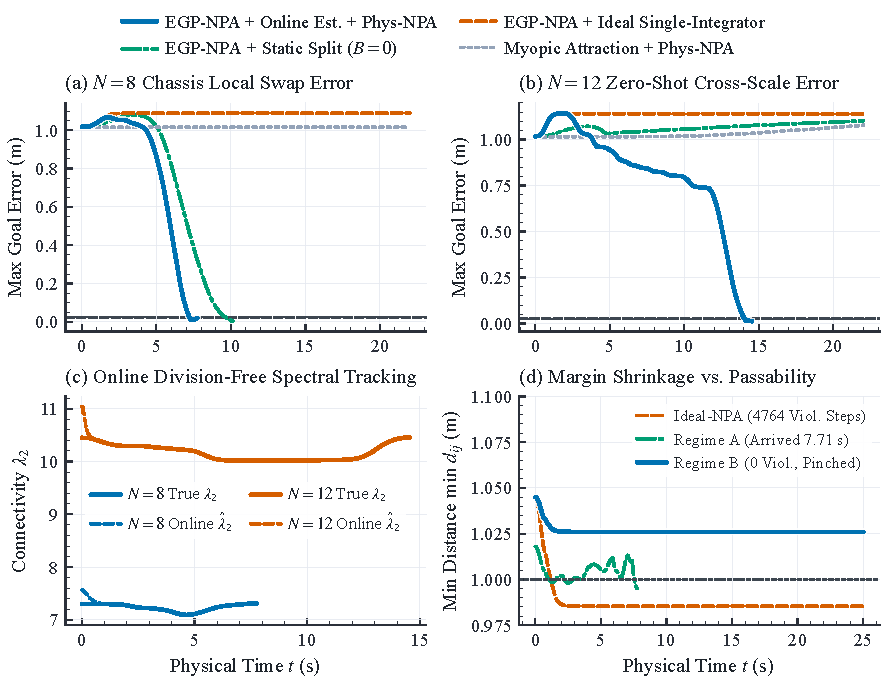
\includegraphics[width=\textwidth]{figures_en/fig6_mujoco_verification.pdf}
 \caption{Full-stack \texttt{MuJoCo} second-order omnidirectional chassis verification combining EGP-NPA, online division-free spectral estimation, and closed-neighborhood NPA. (a)--(b) Maximum goal error on $N=8$ and $N=12$ local swap tasks under Regime~A; (c) real-time $\hat{\lambda}_2(t)$ tracking by the division-free spectral estimator; (d) trade-off between minimum inter-robot clearance $\min d_{ij}(t)$ and channel passability across Ideal-NPA, Regime~A, and Regime~B.}
 \label{fig:mujoco}
\end{figure*}

\begin{theorem}[Critical Channel Pinch-Off Under Physical Margin Shrinkage]\label{thm:passability-tradeoff}
Consider $N$ robots swapping positions on a triangular lattice with initial spacing $S>\ds$, where outer neighbors $j,m$ can open a maximum lateral aperture $d_{jm}^{\max}$. Under physical safety margin shrinkage $\ds^{\mathrm{phys}}=\ds+\Delta d_{\mathrm{phys}}$ ($\mathcal S^{\mathrm{phys}}=\{\bp:\min_{a<b}d_{ab}\ge\ds+\Delta d_{\mathrm{phys}}\}$):
\begin{enumerate}
 \item \textbf{Static initial feasibility:} $\bp(0)\in\operatorname{int}(\mathcal S^{\mathrm{phys}})\Longleftrightarrow \Delta d_{\mathrm{phys}}<S-\ds$.
 \item \textbf{Three-body topological channel pinch-off:} For two counter-crossing robots $i_1,i_2$ passing simultaneously between $j$ and $m$, maintaining pairwise distances $\ge\ds^{\mathrm{phys}}$ at the symmetric midpoint requires a contact rhombus of side length $\ge\ds^{\mathrm{phys}}$, demanding a minimum lateral aperture $d_{jm}^{\mathrm{req}}(\Delta d_{\mathrm{phys}})=\sqrt{3}(\ds+\Delta d_{\mathrm{phys}})$. Whenever $\Delta d_{\mathrm{phys}}>d_{jm}^{\max}/\sqrt{3}-\ds$, the passage undergoes topological pinch-off in $\mathcal S^{\mathrm{phys}}$, disconnecting the initial and target configurations into separate path-connected components of $\mathcal S^{\mathrm{phys}}$.
\end{enumerate}
\end{theorem}
\begin{proof}
Claim (1) follows from $\min_{a<b}d_{ab}(0)=S$. For Claim (2), at the symmetric midpoint, $d_{i_1 i_2}\ge\ds^{\mathrm{phys}}$ and $d_{i_1 j},d_{i_1 m},d_{i_2 j},d_{i_2 m}\ge\ds^{\mathrm{phys}}$ imply $(d_{i_1 i_2}/2)^2+(d_{jm}/2)^2\ge(\ds^{\mathrm{phys}})^2\implies d_{jm}\ge\sqrt{3}(\ds+\Delta d_{\mathrm{phys}})$.
\end{proof}

Table~\ref{tab:mujoco} and Fig.~\ref{fig:mujoco} demonstrate both seamless estimator--policy coupling ($\hat\lambda_2$ RMSE $0.0255\sim 0.0438$ and $0$ connectivity violations across all $64$ runs) and the physical margin--passability trade-off predicted by Theorem~\ref{thm:passability-tradeoff}: under Regime~A ($S=1.018\ \mathrm m$), full-stack EGP-NPA achieves $3/4$ arrivals on $N=8$ and $1/4$ on $N=12$ (vs. $0/8$ for Myopic and Ideal-NPA), whereas enforcing $\Delta d_{\mathrm{phys}}=0.028\ \mathrm m$ under Regime~B eliminates soft-boundary grazing ($0$ violations on $7/8$ tasks) at the cost of pinching off the three-body swap channels.
